%!TEX root = ../../main.tex


\begin{figure}[p]
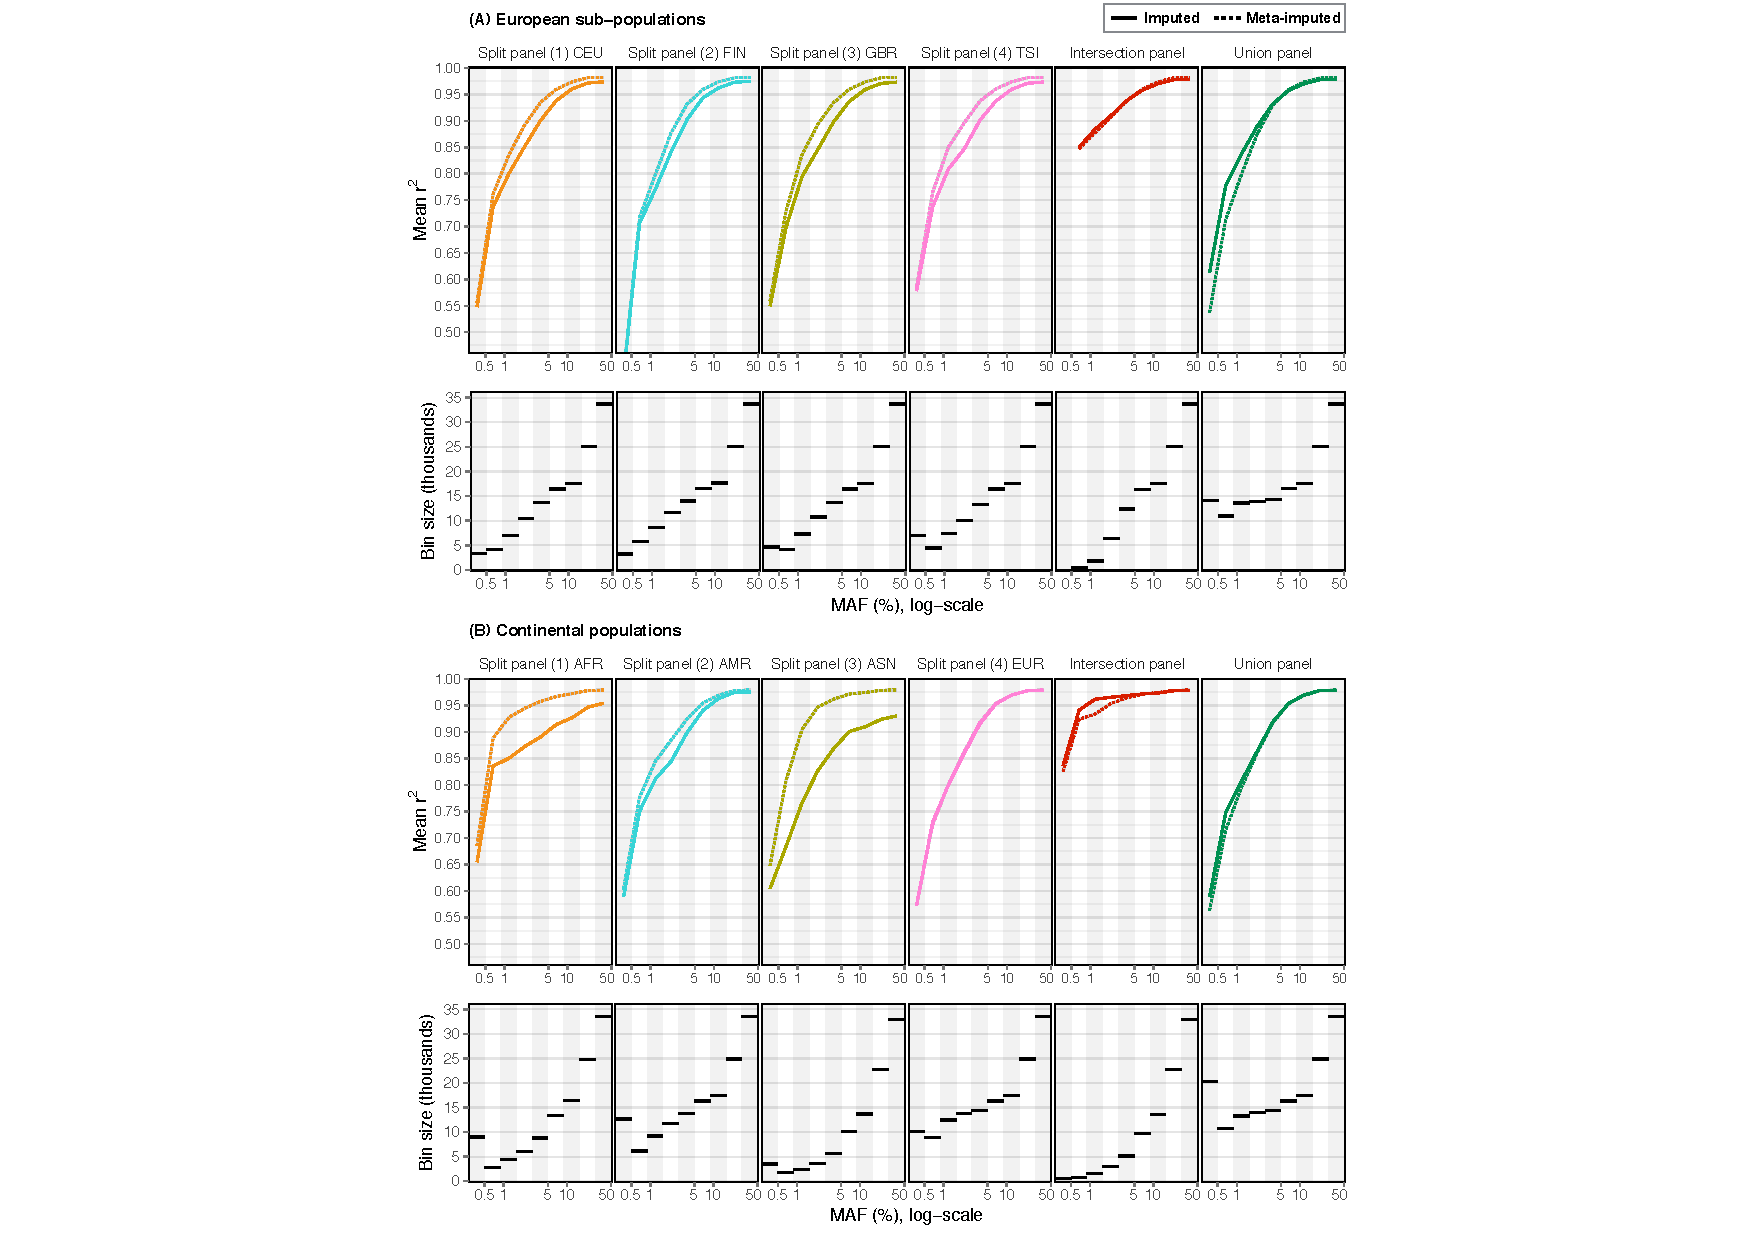
\includegraphics[width=\textwidth]{./img/ch2/accuracy_imp_maf_rsq}
\Caption{Accuracy comparison between meta-imputation and direct imputations}
{Accuracy was measured as mean~$r^2$ per \gls{maf} bin, defined on log-scale where \emph{grey-white} bars indicate boundaries.
Each imputed panel (imputations from the \n{4} split panels, the intersection panel, and the union panel) was separately compared to meta-imputation on the same set of variants per bin; shown for variants retained after \gls{qc}, in Scenarios~A and B.
\Gls{maf} bins were defined on the actual allele frequencies as determined by the \gls{got2d} dataset.
Note that mean~$r^2$ is not shown if the number of markers dropped below \n{50} per \gls{maf} bin.
Panels at the bottom show the number of variants compared per bin.}
{fig:imp_rsq}
\end{figure}
